\begin{center}
 \textsc{Физбой, 10 класс. Полуфинал.}
\end{center}
\vspace{0.01cm}
\hrule
\parindent=0mm

\task{ Тело начинает движение из точки $A$ и движется сначала
  равноускоренно в течение времени $T_0$, затем с тем же по модулю
  ускорением --- равнозамедленно. Через какое время от начала движения
  тело вернется в точку $A$?}

\task{Легкая нерастяжимая нить длиной $2 \unit{м}$ удерживается за
   ее концы так, что они находятся на данной высоте рядом друг с
   другом. На нити висит проволочная скобка в виде перевернутой буквы
   U. Масса скобки равна 1 грамму. Нить выдерживает максимальную
   растягивающую силу $F = 5 \unit{Н}$. ($F \gg mg$). Концы нити
   начинают перемещать в противоположных горизонтальных направлениях с
   одинаковыми скоростями $1 \unit{м/с}$. В какой-то момент нить не
   выдерживает и рвется. На какую максимальную высоту в момент разрыва
   нити взлетит скобка? Сопротивлением воздуха пренебречь.}

 \task{ Две бесконечные пластины толщины $h$ заряжены равномерно по
   объему и сложены вместе. Объемная плотность заряда первой пластины
   $\rho$, а второй $-\rho$. Найдите максимальную напряженность
   электрического поля. }

 \taskpic{ В чёрном ящике находится резистор, имеющий постоянное
   сопротивление и нелинейный элемент, которые могут быть включены как
   последовательно, так и параллельно. Найдите сопротивление
   резистора. Какой нелинейный элемент может находиться внутри чёрного
   ящика? ВАХ для последовательно и параллельно включеных элементов
   представлены на рисунке.}{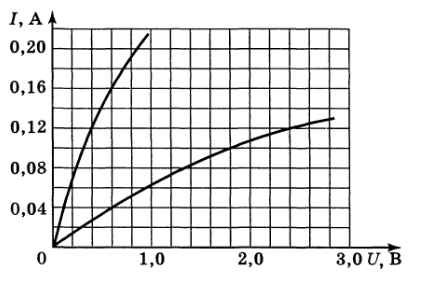
\includegraphics[width=4cm]{fb10_s_1.png}}

 \task{ В чайник с нагревательным элементом мощностью $P$ = 2200 Вт
   налили $V_1 = 1.5 \mbox{ л}$ холодной воды и включили его. когда
   вода закипела, он автоматически отключился. Через $t_1 = 60 \mbox{
     с}$ его снова включили, а еще через $t_2 = 6 \mbox{ с}$ вода
   закипела и чайник выключился. сразу после этого его еще раз
   включили, но сняв крышку. Автоматический выключатель, срабатывающий
   под давлением пара, перестал действовать, и вода из чайника начала
   выкипать. Через $t_3 = 240 \mbox{ с}$ после последнего включения
   измерили объем оставшейся воды. Он оказался равным $V_2 = 1.3
   \mbox{ л}$. Каково значение удельной теплоты парообразования воды
   $L$?  Удельная теплоемкость воды $c = 4200 \mbox{ Дж/(кг*К)}$,
   плотность $\rho = 1000 \mbox{ кг/м}^3$. Теплоемкостью чайника
   пренебречь.}

 \taskpic{ Говорят, что в архиве Снеллиуса нашли рисунок с оптической
   схемой. От времени чернила выцвели, и на бумаге остались видны
   только предмет и его изображение, даваемое тонкой линзой.\\
   1) восстановите построением по имеющимся данным положение линзы.\\
   2) найдите положение фокусов линзы.  \\
   3) можно ли, исходя из рисунка, сказать, какая (собирающая или рассеивающая) была линза?  }{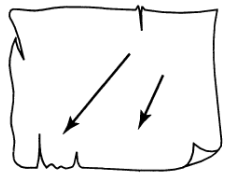
\includegraphics[width=4cm]{fb10_s_6.png}}
\setcounter{notask}{1}
